\section{Versuchsdurchführung}
\subsection{Versuchsapparate}
Für die Widerstandsmessung stehen ein Multimeter und eine Leiterprobe vorgegebener Länge zur Verfügung. 
Längenmessungen werden mit einer Micrometerschraube vorgenommen. Für die Messung der Hall-Spannung steht 
ein Elektromagnet \autoref{fig:emagnet} zur verfügung, der aus zwei in Reihe geschalteten Spulen besteht, zwischen denen die 
Leiterprobe platziert werden kann. Sowohl die Probe als auch die Spulen werden durch ein Konstantstromgerät 
gespeist. Für die Messung der magnetischen Feldstärke steht ein Teslameter zur verfügung, sowie für die 
Hall-Spannung ein Voltmeter mit hoher Auflösung.
\begin{figure}
    \centering
    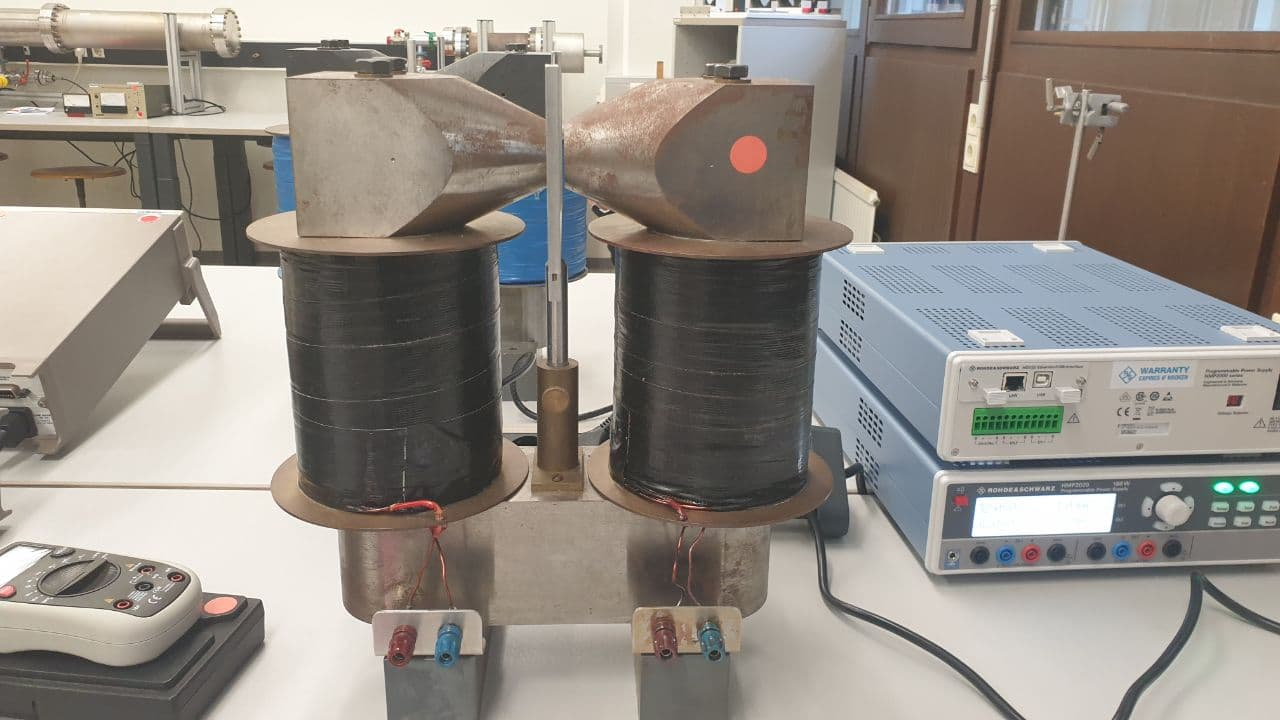
\includegraphics[width=10cm]{magnet.png}
    \caption{Elektromagnet}
    \label{fig:emagnet}
  \end{figure}

  \begin{figure}
    \centering
    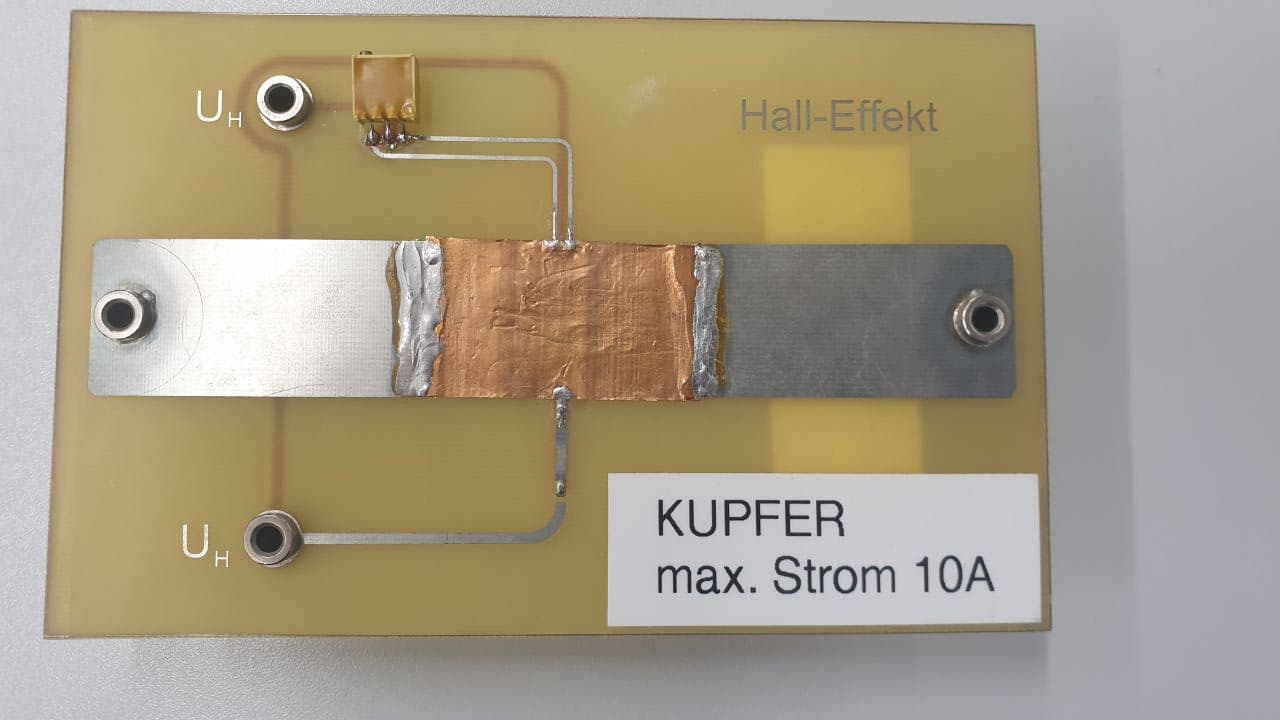
\includegraphics[width=10cm]{probe.png}
    \caption{Folienprobe}
    \label{fig:probe}
  \end{figure}
\subsection{Messung des Widerstandes}
Zur Widerstandsmessung wurde das Multimeter an den bereitgestellten Draht angeschlossen, sodass der 
Widerstandswert abgelesen werden konnte. Anschließend wurden mithilfe des Micrometers der Durchmesser 
des Drahtes sowie Länge, Breite und Dicke der Leiterplatte \autoref{fig:probe} jeweils an separaten zur Längenmessung 
bereitgestellten Proben gemessen.
\subsection{Messung der Hall-Spannung}
Für die Messung der Hall-Spannung wurde zunächst eine Messreihe für die magnetische Feldstärke durchgeführt. Dafür wurde das Teslameter im Magnetfeld des Elektromagneten ausgerichtet und anschließend der Spulenstrom am Kontaktstromgerät
beginnend mit $0,5A$ bis zum Wert $4,5A$ jeweils in Intervallen von $0,5A$ erhöht und die zugehörige Feldstärke notiert, anschließend wurde die Polung des Megnetfeldes umgekehrt und das Vorgehen wiederholt. Danach wurden zwei Messreihen für die Hall-Spannung durchgeführt. in der ersten Messreihe wurde bei konstantem Probenstrom der Spulenstrom nach dem gleichen Muster wie bei der vorangegangenen Messreihe variirt und die abfallende Hall-Spannung gemessen. Auch hier wurden identische Messriehen für beide Polungen durchgeführt. Dabei wurde wie bei allen Messungen der Spulenstrom vor dem abschalten heruntergeregelt, um einen plötzlich auftretenden Induktionsspannungsstoß zu vermeiden. In der letzten Messreihe wurde bei einem konstanten Spulenstrom von $4A$ der Probenstrom variirt und die Hall-Spannung gemessen. Auch hier wurde die Messung für beide Polungen durchgeführt. Die Werte des Probenstroms wurden wie in den vorangegangenen Messreihen variirt, jedoch aufgrund des Konstantstromgerätes nur bis zum Wert $2,5A$. 
